\begin{BPMN}{PROC-04}{Carga del Mapa Curricular}{fsnkjfnwkjlfnkawn}
    \PCitem{Participantes}{
    	\begin{itemize}
    		\item Jefe de Innovación Educativa
    		\item Jefe de División de Innovación Académica
    		\item Jefe de Departamento de Desarrollo e Innovación Curricular
    		\item Analista DES
    	\end{itemize}
    }
    \PCitem{Objetivo}{Subir la información contenida en el Mapa Curricular para asistir en la elaboración y revisión de los Programas de Estudio}
    \PCitem{Interrelación con otros procesos}{
        \begin{itemize}
            \item Entrada: Recibir respuesta de aprobación del Plan de Estudios
            \item Salida: Elaborar Unidades de Aprendizaje
        \end{itemize}
    }
    \PCitem{Proveedores}{Dirección de Educación Superior}
    \PCitem{Entradas}{Aprobación del Plan de Estudios}
    \PCitem{Consumidores}{Unidad Académica}
    \PCitem{Salidas}{}
    \PCitem{Precondiciones}{Elaboración y Aprobación del Plan de Estudios}
    \PCitem{Postcondiciones}{Elaboración de Unidade de Aprendizaje}
    \PCitem{Frecuencia}{}
    \PCitem{Tipo}{Operación}
\end{BPMN}
\hypertarget{SP4}{\begin{figure}[htbp]
	\begin{center}
	%\includegraphics[width=.95\textwidth]{C1-DP/SP4/Image/CasosDeUsoSP4}
		%\caption{UML-04 Casos de uso para la  Elaboración del Plan de Estudios}
		%\label{fig:CDU-04}
	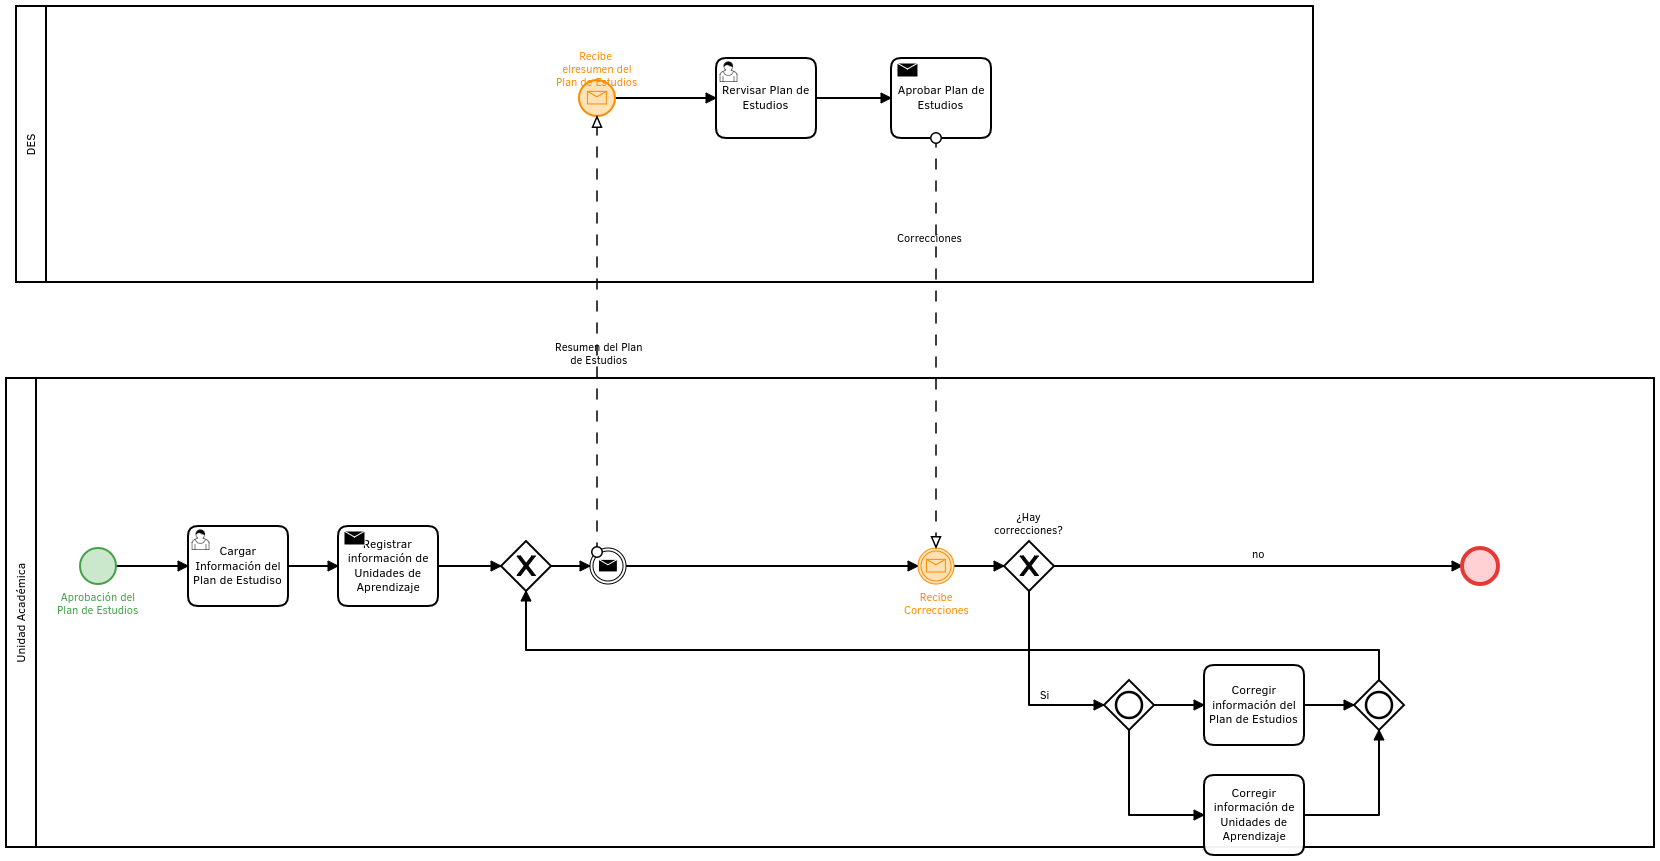
\includegraphics[width=.95\textwidth]{C1-DP/SP4/Image/SP4}
		\caption{BPMN-04 Subproceso para la carga del Mapa Curricular}
		\label{fig:BPMN-04}
	\end{center}
\end{figure}}